\documentclass[11pt]{article}
\usepackage[margin=1in]{geometry}
\usepackage{amsmath,amssymb,amsthm,booktabs,graphicx,microtype}
\usepackage[colorlinks=true,linkcolor=blue!50!black,urlcolor=blue!50!black,citecolor=blue!50!black]{hyperref}
\usepackage{xcolor}
\usepackage{xurl}
\setlength{\emergencystretch}{2em}
\usepackage{fancyhdr}
\pagestyle{fancy}\fancyhf{}\fancyhead[L]{\small Boundary traces and derivative constraints}\fancyhead[R]{\small S. Gupta}\fancyfoot[C]{\thepage}
\setlength{\headheight}{14pt}
\newtheorem{theorem}{Theorem}
\newtheorem{proposition}[theorem]{Proposition}
\newtheorem{corollary}[theorem]{Corollary}
\newcommand{\PP}{\mathcal P}
\newcommand{\proj}{\Pi_p}
\newcommand{\ip}[2]{\langle #1,#2\rangle}
\newcommand{\norm}[1]{\lVert #1\rVert}
\title{Two Boundary Traces Determine Derivative-Constraint\newline Injection in Legendre \(p\)-Coarsening}
\author{Shivam Gupta\\\small Independent Researcher\\\small\href{mailto:shivam1720406@gmail.com}{shivam1720406@gmail.com}}
\date{17 October 2026}
\begin{document}
\maketitle
\begin{abstract}
First-order wave formulations evolve a field and its spatial derivative as independent variables. Reducing their polynomial degrees independently can therefore create a reduction-constraint violation. For exact, unweighted Legendre projection on an affine interval, we express the entire injected constraint using only the two endpoint values of the discarded field. This factorization gives an exact constraint norm and sharp finite-band singular values, and shows why constraint injection need not decrease monotonically with the retained degree. We then express the standard nearest compatible graph projection as two cached boundary responses for consistent source data. A polynomial counterexample shows that resetting the derivative of the truncated field can increase the specified pair norm by a factor of \(320/231\), whereas graph projection is contractive in that norm. Reproducible tests comprise 2,880 transfer cases, independent quadrature-based verification, smooth-profile approximation, and 54 periodic scalar-wave discontinuous Galerkin runs. The evolution results also establish a limitation: eliminating the local transfer constraint does not guarantee lower subsequent solution error or constraint violation. The resulting diagnostic separates transfer consistency from evolution accuracy and provides a small, explicit test case for adaptive first-order wave codes.
\end{abstract}
\noindent\textbf{Keywords:} spectral adaptivity; reduction constraints; Legendre projection; discontinuous Galerkin; first-order wave systems.

\section{Introduction}
Spectral adaptivity changes both the resolution and the representation of a numerical state. For a first-order reduction, the components of that state are related by differential identities. In the scalar example, a field \(\psi\) and an auxiliary field \(\Phi\) satisfy
\begin{equation}\label{eq:constraint}
 C=\partial_x\psi-\Phi=0.
\end{equation}
The generalized harmonic formulation similarly includes reduction constraints relating spatial derivatives of the metric to auxiliary variables \cite{lindblom}. Spectral adaptive mesh refinement is an established ingredient of SpEC \cite{szilagyi}, and SpECTRE provides spectral projection infrastructure for numerical-relativity calculations \cite{kidder,spectre}. A transfer operation should consequently be assessed for its effect on differential consistency as well as its approximation error.

Consider a polynomial \(f\) of degree \(q\), its derivative \(f'\), and an exact \(L^2(-1,1)\) projection \(\proj\) onto degree \(p<q\). Fieldwise projection produces \((\proj f,\proj f')\). Its reduction constraint is the negative of
\begin{equation}\label{eq:commutator}
 J_p f=\proj f'-(\proj f)'.
\end{equation}
The practical question is whether one must analyze a full transfer matrix to determine this defect. On an affine Legendre element, the answer is no: two discarded-tail endpoint sums determine it exactly. Their cancellation can hide a substantial discarded field while making \(J_pf\) vanish. The diagnostic is therefore exact for transfer consistency but insufficient as an accuracy estimator.

This paper develops that distinction. We derive the boundary factorization, its exact norm, and its two possible nonzero singular values. We use the same data to implement a classical graph projection through cached responses. Finally, we compare independent projection, derivative reset, and graph projection both at transfer and in a subsequent scalar-wave evolution. The experiments deliberately retain outcomes unfavorable to compatible transfer. They show why a local constraint guarantee must not be interpreted as an accuracy or stability guarantee for a complete evolution scheme.

\paragraph{Relationship to established methods.}
Optimal constraint projection is established in numerical relativity, including scalar-field tests on black-hole backgrounds \cite{holst}. The projection used here is a finite-dimensional specialization of that principle. Polynomial differentiation and truncation are also known not to commute; explicit Legendre differentiation formulas appear, for example, in Rapisarda et al.\ \cite{rapisarda}. Boundary lifts are standard in DG and flux reconstruction \cite{huynh}; efficient Legendre variational solvers and adaptive spectral coarsening have a long history \cite{shen,canuto}. We do not claim these general ideas as new. The contribution is the explicit two-trace transfer diagnostic with sharp finite-band amplification, its consequences for degree selection, and a reproducible comparison that separates local compatibility from later wave accuracy. The proofs use classical polynomial identities. The literature review supports this focused positioning rather than a claim of absolute priority for every identity.

\section{Exact boundary representation}
Let \(P_n\) be the Legendre polynomial normalized by \(P_n(1)=1\). Set \(\PP_p=\operatorname{span}\{P_0,\ldots,P_p\}\), with the unweighted inner product on \([-1,1]\). The exact modal mass entries are
\begin{equation}\label{eq:mass}
 m_n=\ip{P_n}{P_n}=\frac{2}{2n+1}.
\end{equation}
For \(f\in H^1(-1,1)\), define the discarded residual \(r=f-\proj f\) and its two traces \(t_+=r(1)\), \(t_-=r(-1)\). In one dimension these traces are well defined. Define the reproducing endpoint kernels
\begin{equation}
 K_p(x,s)=\sum_{k=0}^p\frac{2k+1}{2}P_k(x)P_k(s),\qquad s\in\{-1,1\}.
\end{equation}

\begin{theorem}[Two-trace factorization]\label{thm:trace}
For every \(f\in H^1(-1,1)\),
\begin{equation}\label{eq:trace}
 J_pf=t_+K_p(x,1)-t_-K_p(x,-1).
\end{equation}
In particular, the modal coefficient of \(P_k\) is
\begin{equation}\label{eq:coeff}
 (J_pf)_k=\frac{2k+1}{2}\bigl(t_+-(-1)^kt_-\bigr).
\end{equation}
For \(p\geq1\), the operator \(J_p\) has rank two on \(H^1(-1,1)\). On \(\PP_q\) with \(q>p\), its rank is one if \(q=p+1\), and two if \(q\geq p+2\).
\end{theorem}
\begin{proof}
Since \((\proj f)'\in\PP_p\), we have \(J_pf=\proj r'\). For any \(v\in\PP_p\), integration by parts gives
\begin{equation}
 \ip{J_pf}{v}=r(1)v(1)-r(-1)v(-1)-\ip{r}{v'}.
\end{equation}
The last term vanishes because \(v'\in\PP_{p-1}\) and \(r\) is orthogonal to \(\PP_p\). The endpoint kernels represent the remaining two functionals, proving \eqref{eq:trace}. Their coefficient vectors are independent for \(p\geq1\). The residual polynomials \(P_{p+1}\) and \(P_{p+2}\) have independent endpoint pairs, proving the rank statements. For \(q=p+1\), only the first residual polynomial is available.
\end{proof}

\begin{corollary}[Exact injected norm]\label{cor:norm}
Writing \(N=p+1\), the squared defect is
\begin{equation}\label{eq:exactnorm}
 \norm{J_pf}^2=\frac{N^2}{2}(t_+^2+t_-^2)-(-1)^pN t_+t_-.
\end{equation}
The eigenvalues of this quadratic form are \(Np/2\) and \(N(p+2)/2\).
\end{corollary}
\begin{proof}
Orthogonality and \eqref{eq:coeff} reduce the norm to a sum of \((2k+1)(t_+-(-1)^kt_-)^2/2\). Use \(\sum_{k=0}^p(2k+1)=N^2\) and \(\sum_{k=0}^p(-1)^k(2k+1)=(-1)^pN\). The two diagonal entries of its matrix are \(N^2/2\), and the off-diagonal entries are \(-(-1)^pN/2\).
\end{proof}

\subsection{Sharp amplification of a finite discarded band}
The exact norm also admits a sharp interpretation relative to the discarded \(L^2\) mass. Suppose \(f\in\PP_q\), and define the retained index sets \(I_a=\{0\leq k\leq p:k\equiv a\pmod2\}\) and discarded sets \(T_a=\{p<n\leq q:n\equiv a\pmod2\}\), for \(a\in\{0,1\}\).

\begin{proposition}[Finite-band singular values]\label{prop:sv}
In orthonormal modal coordinates, the two possible nonzero singular values of the map from the discarded band to \(J_pf\) are
\begin{equation}\label{eq:sv}
 \sigma_a=\left(\sum_{k\in I_a}(2k+1)\sum_{n\in T_{1-a}}(2n+1)\right)^{1/2},\qquad a=0,1.
\end{equation}
Empty sums give zero. Thus \(\norm{J_pf}\leq\max_a\sigma_a\norm{r}\), with equality attained by an appropriate discarded polynomial.
\end{proposition}
\begin{proof}
The Legendre derivative matrix satisfies \(D_{kn}=2k+1\) when \(n>k\) and \(n-k\) is odd, and is zero otherwise. Restricted to \(k\leq p<n\), its orthonormal-coordinate entries are \(\sqrt{(2k+1)(2n+1)}\) for opposite parities. After grouping parity, the matrix has two disjoint rank-one blocks, each an outer product. Their singular values are the products of the Euclidean norms of the two vectors, yielding \eqref{eq:sv}. A right singular vector gives equality.
\end{proof}

\subsection{Why degree selection is not monotone}
Let \(f=P_9-P_{11}\). For every \(p<9\), the discarded residual has both endpoint traces zero, so \(J_pf=0\). At \(p=9\), only \(-P_{11}\) remains discarded, and \(J_pf\ne0\); once \(p\geq11\), the defect vanishes again. Consequently, binary search on an assumed monotone injection tolerance is invalid. This example also proves that zero injection is not an accuracy certificate: at \(p<9\), the entire nonzero function is discarded. An adaptive algorithm must combine a consistency test such as \eqref{eq:exactnorm} with an independent approximation-error test. Scanning all candidate degrees requires only suffix sums of even and odd coefficients and suffix sums of modal mass.

\begin{figure}[t]
 \centering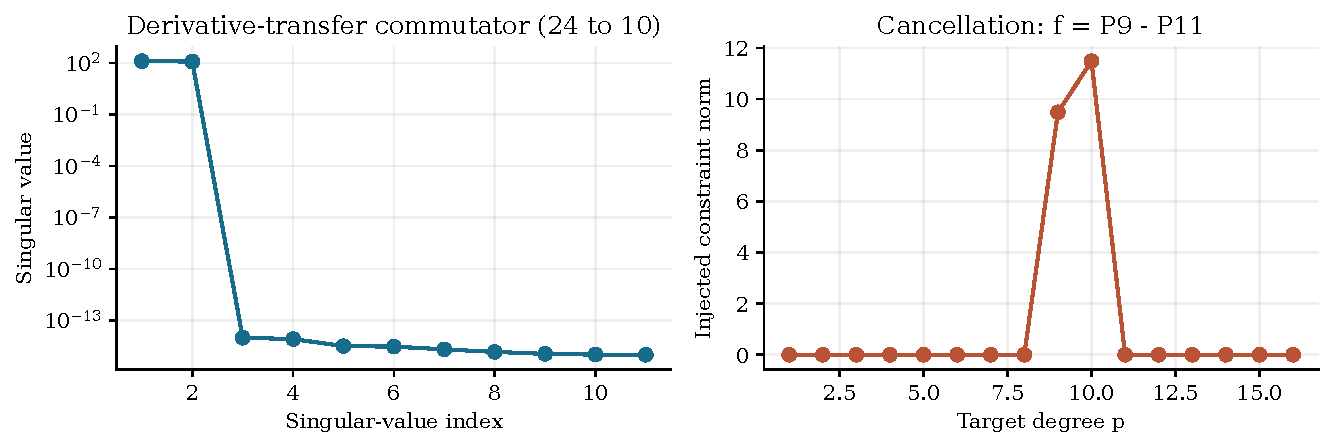
\includegraphics[width=\linewidth]{../figures/boundary.pdf}
 \caption{The exact-mass derivative-transfer commutator has two nonzero singular values (left; the remaining values are at floating-point roundoff). Its norm can increase when more modes are retained (right), because discarded endpoint contributions can cancel. Both panels are generated from the stated polynomial operators.}\label{fig:boundary}
\end{figure}

\subsection{Existing constraints and tensor products}
For an arbitrary source pair \((f,g)\), let \(C=f'-g\). Independent projection obeys the exact decomposition
\begin{equation}\label{eq:oldnew}
 (\proj f)'-\proj g=\proj C-J_pf.
\end{equation}
Thus the two traces determine the newly injected part, not the full constraint for an already inconsistent source. Applying the consistent-source shortcut to inconsistent data would ignore \(\proj C\).

On a Cartesian tensor-product element, let \(\Pi=\Pi_p^{\otimes d}\). For differentiation in direction \(i\), first project tangentially and apply Theorem~\ref{thm:trace} in the normal coordinate. The defect depends on two face polynomials of tangential degree at most \(p\). Therefore its rank is at most \(2(p+1)^{d-1}\), and equals this value for \(p\geq1\) if the source tensor degree is at least \(p+2\) in the normal direction. Independence follows by multiplying either of the two normal residual polynomials by each retained tangential basis function. This is a face-data result, not two scalar numbers for an entire three-dimensional element. The accompanying tests verify the two-dimensional rank algebraically; all evolution experiments below remain one dimensional.

\section{Compatible transfer and its costs}
Three natural transfers have distinct objectives. Independent projection gives the best unconstrained pair approximation. Derivative reset retains \(u=\proj f\) and assigns \(v=u'\). Graph projection instead chooses \(u\in\PP_p\) to minimize
\begin{equation}\label{eq:objective}
 \mathcal E_\ell(u)=\norm{u-f}^2+\ell^2\norm{u'-g}^2,\qquad \ell>0,
\end{equation}
and returns \((u,u')\). The parameter \(\ell\) sets the relative importance of the auxiliary derivative; it is part of the specified transfer norm, not an empirically optimized physical parameter. For a physical element of width \(h\), a physical-unit pair norm with equal field weights corresponds to \(\ell=2/h\) after converting the physical derivative to the logical derivative.

Let \(M=\operatorname{diag}(m_0,\ldots,m_p)\), and let \(D\) be the degree-\(p\) modal derivative matrix. Put \(a=\proj f\), \(b=\proj g\) in modal coordinates. The unique minimizer solves
\begin{equation}\label{eq:normal}
 H_\ell u=Ma+\ell^2D^TMb,\qquad H_\ell=M+\ell^2D^TMD.
\end{equation}
Positive definiteness follows from \(M>0\). This is the familiar finite-dimensional Sobolev/graph projection, consistent with the nearest-constraint-state principle of \cite{holst}.

\begin{proposition}[Two cached responses]\label{prop:response}
If \(g=f'\), let \(L\) be the \((p+1)\)-by-2 coefficient matrix in \eqref{eq:coeff}, and \(t=(t_+,t_-)^T\). Then
\begin{equation}\label{eq:response}
 u=a+B_\ell t,\qquad B_\ell=H_\ell^{-1}\ell^2D^TML.
\end{equation}
The source polynomial influences the correction only through its two discarded traces. The constant coefficient of \(u\) equals that of \(f\).
\end{proposition}
\begin{proof}
Theorem~\ref{thm:trace} gives \(b=Da+Lt\). Substitute this into \eqref{eq:normal} and subtract \(H_\ell a\). The first column of \(D\) is zero, so the first row and column of \(D^TMD\) are zero; the correction's constant coefficient consequently vanishes.
\end{proof}

For a fixed degree and \(\ell\), the two columns of \(B_\ell\) can be cached. Tail evaluation costs \(O(q-p)\), and evaluating \(u\) from \eqref{eq:response} costs \(O(p)\). Differentiation can use the standard linear-cost Legendre recurrence. The reference implementation uses dense differentiation matrices for clarity, so its complete transfer still costs \(O(p^2)\). We report no production speedup. For inconsistent data, \eqref{eq:normal} remains valid; the general implementation uses it instead of \eqref{eq:response}.

\begin{proposition}[Local contractivity]\label{prop:contract}
Define \(\norm{(f,g)}_\ell^2=\norm f^2+\ell^2\norm g^2\). Graph projection is an orthogonal projection onto the linear subspace \(G_p=\{(u,u'):u\in\PP_p\}\) of the pair space. Hence
\begin{equation}\label{eq:pythagoras}
 \norm{(f,g)}_\ell^2=\norm{(u,u')}_\ell^2+\mathcal E_\ell(u).
\end{equation}
It is contractive in this pair norm and minimizes transfer error among compatible target pairs.
\end{proposition}
\begin{proof}
The stationarity condition for \eqref{eq:objective} is orthogonality of the residual to every \((v,v')\in G_p\). Since the minimizer is in \(G_p\), the Pythagorean identity follows. The same orthogonality gives the best-approximation property.
\end{proof}

The guarantee concerns a single transfer. The term \(\norm f^2\) is included in this norm, whereas the usual flat-space scalar-wave energy uses the time derivative and spatial derivative. Equation~\eqref{eq:pythagoras} is neither conservation of physical wave energy nor a stability theorem for an evolution method. It also does not preserve endpoint values, derivative means, or characteristic interface data in general.

\subsection{Reset can increase the pair norm}
Take \(f=P_2-\tfrac3{10}P_4\), \(g=f'\), \(p=2\), and \(\ell=1\). Orthogonality gives \(\norm f^2=21/50\), \(\norm{f'}^2=21/5\), and therefore \(\norm{(f,f')}_1^2=231/50\). Reset returns \((P_2,P_2')\), with squared pair norm \(32/5\). Its norm-squared ratio is
\begin{equation}\label{eq:counter}
 \frac{32/5}{231/50}=\frac{320}{231}\simeq1.38528.
\end{equation}
Cancellation in the derivative of the discarded mode is lost. Graph projection is contractive by Proposition~\ref{prop:contract}; independent projection is contractive in the unconstrained pair space but generally violates \eqref{eq:constraint}. These are different guarantees, and none alone selects the most accurate subsequent trajectory.

\section{Reproducible numerical study}
All experiments use IEEE double precision. The reference environment is Python 3.9.6, NumPy 1.26.4, SciPy 1.13.1, and Matplotlib 3.9.4. Code, raw CSV data, tests, vector figures, and manuscript sources are available at \url{https://github.com/shi1720/legendre-constraint-coarsening}. No external data are required.

\subsection{Algebraic verification and independent checks}
We draw coefficients \(a_n=z_n/(n+1)^2\), with independent standard normal \(z_n\), using seed 6602027. Source degrees are \(q\in\{8,16,24,32,48\}\); target degrees are the distinct values in \(\{1,2,4,\lfloor q/2\rfloor,q-1\}\). Each valid degree pair is tested at \(\ell\in\{0.03,0.3,3\}\) with 40 draws, giving 2,880 cases. The source auxiliary field is the exact polynomial derivative.

Table~\ref{tab:algebra} reports normalized residuals, using \(1+\norm{\cdot}\) or \(1+|\cdot|\) in the denominator to avoid division by a vanishing reference. The largest graph norm-squared ratio was below one up to roundoff, while reset reached 1.23071 in this ensemble. The explicit counterexample \eqref{eq:counter} is stronger and does not depend on random sampling. Graph error never exceeded reset error in the tested cases, as required by best approximation within \(G_p\).

\begin{table}[t]\centering
\caption{Maximum normalized residual across 2,880 transfer cases. These are numerical checks of exact identities, not estimates of physical modeling error.}\label{tab:algebra}
\begin{tabular}{lr}\toprule
Identity checked & Maximum residual\\\midrule
Boundary factorization \eqref{eq:trace} & \(4.26\times10^{-16}\)\\
Exact defect norm \eqref{eq:exactnorm} & \(2.59\times10^{-16}\)\\
Cached response vs. general normal solve & \(2.13\times10^{-16}\)\\
Pair-norm Pythagorean identity & \(7.65\times10^{-16}\)\\\bottomrule
\end{tabular}
\end{table}

Nine automated tests cover differentiation against NumPy's independent polynomial routine, boundary factorization, the two singular values, a tensor face rank, trace cancellation, the reset counterexample, inconsistent-source decomposition, projection optimality, and independent quadrature verification. For the last check, Gauss--Legendre quadrature constructs a stacked least-squares system for field values and derivatives; a least-squares solver is compared with \eqref{eq:normal} for both consistent and arbitrary source pairs. Degree pairs are \((q,p)=(8,3),(20,7),(32,16)\), with \(\ell=0.03,1,30\). This checks a different assembly and solver path rather than merely evaluating the same matrix formula twice.

\subsection{Smooth approximation}
We project \(\sin(3x+0.3)\), \(\exp[-20(x-0.17)^2]\), and \(\exp[8(x-1)]\) to source degree 48 using 96-point Gauss quadrature, differentiate the resulting source polynomial, and transfer to degrees 2 through 24. Errors in Figure~\ref{fig:analytic} are measured against that degree-48 source pair, with \(\ell=1\). They are transfer errors, not errors against the unprojected analytic derivative. Independent projection has the smallest pair error because it has no compatibility restriction. Graph projection is optimal among compatible pairs; reset is another compatible pair and can only match or exceed its transfer error. The observed approach to roundoff for the analytic profiles is consistent with spectral approximation, but the construction does not establish a uniform convergence theorem for arbitrary nonsmooth data.

\begin{figure}[t]\centering
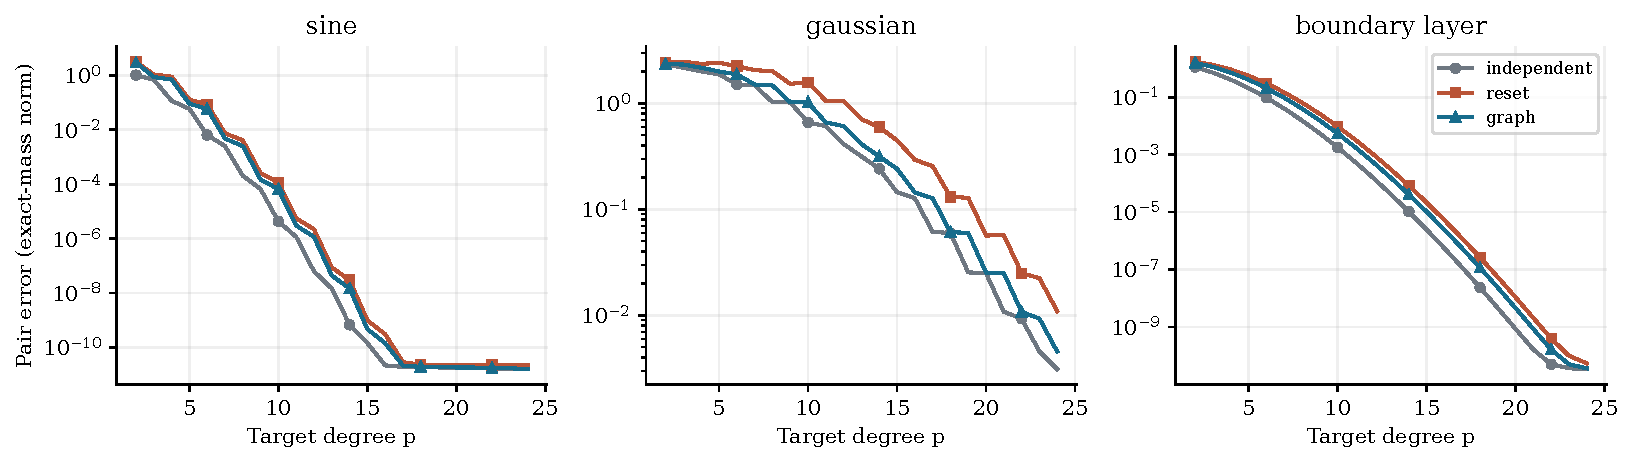
\includegraphics[width=\linewidth]{../figures/analytic.pdf}
\caption{Transfer error for three smooth source profiles. Independent projection minimizes error in the full pair space; graph projection minimizes error in its compatible subspace. The distinction matters when assessing a constraint-preserving transfer.}\label{fig:analytic}
\end{figure}

\subsection{A periodic scalar-wave evolution test}
We evolve
\begin{equation}\label{eq:wave}
 \psi_t=-\pi,\qquad \pi_t=-\partial_x\Phi,\qquad \Phi_t=-\partial_x\pi
\end{equation}
on \([0,2\pi]\), with periodic boundaries and exact solution \(\psi=\sin(x-t)\), \(\pi=\Phi=\cos(x-t)\). We use 4, 8, or 16 equal elements, exact modal masses, and a strong-form upwind DG discretization for \((\pi,\Phi)\). If \(U=(\pi,\Phi)^T\) and \(A=\left(\begin{smallmatrix}0&1\\1&0\end{smallmatrix}\right)\), the interface flux is
\begin{equation}
 F^*(U^-,U^+)=\tfrac12 A(U^-+U^+)-\tfrac12(U^+-U^-).
\end{equation}
The field \(\psi\) obeys the element-local equation in \eqref{eq:wave}. Classical fourth-order Runge--Kutta advances the state. Source degree 10 is evolved to \(t=0.2\), transferred once to degree 3, 5, or 7, and evolved to \(t=0.5\). The time-step bound is \(0.02h/(p+1)^2\), with a uniform step reduced as necessary to reach each specified time exactly. Every post-transfer evolution is repeated at half that time step. There are 54 post-transfer runs; the pre-transfer stage is shared for each element count. Three additional uncoarsened degree-10 controls check the underlying evolution against the same analytic solution; their final field errors are \(2.69\times10^{-11}\), \(7.46\times10^{-14}\), and \(5.01\times10^{-14}\), respectively.

Independent transfer truncates each of the three fields. Reset truncates \(\psi,\pi\) and sets \(\Phi=(2/h)D\psi\). Graph transfer minimizes the physical pair error for \((\psi,\Phi)\), using \eqref{eq:normal} to accommodate any source inconsistency; \(\pi\) is projected independently. The final three-field error is integrated against the analytic solution with 40-point Gauss quadrature. Constraint norms use the local polynomial derivative, without a DG interface lift.

\begin{table}[t]\centering\small
\caption{Degree-10 to degree-3 scalar-wave runs, using the smaller time step. \(E=\norm{(\psi,\pi,\Phi)-(\psi_*,\pi_*,\Phi_*)}_{L^2}\) at \(t=0.5\); \(C\) is the final local reduction-constraint norm.}\label{tab:wave}
\begin{tabular}{rlrr}\toprule
Elements & Transfer & \(E\) & \(\norm C\)\\\midrule
4 & Independent & \(4.8322\times10^{-3}\) & \(2.4890\times10^{-2}\)\\
4 & Reset & \(1.1368\times10^{-2}\) & \(2.2846\times10^{-2}\)\\
4 & Graph & \(1.1595\times10^{-2}\) & \(2.0756\times10^{-2}\)\\\addlinespace
8 & Independent & \(3.4237\times10^{-4}\) & \(3.2512\times10^{-3}\)\\
8 & Reset & \(9.2521\times10^{-4}\) & \(3.0315\times10^{-3}\)\\
8 & Graph & \(1.2218\times10^{-3}\) & \(3.4767\times10^{-3}\)\\\addlinespace
16 & Independent & \(2.1146\times10^{-5}\) & \(4.1336\times10^{-4}\)\\
16 & Reset & \(6.9464\times10^{-5}\) & \(4.4241\times10^{-4}\)\\
16 & Graph & \(1.3157\times10^{-4}\) & \(4.3739\times10^{-4}\)\\\bottomrule
\end{tabular}
\end{table}

Reset and graph transfers reduce the immediate local constraint to below \(3\times10^{-16}\) in the degree-3 runs. Yet independent transfer has the smallest final solution error in every row group of Table~\ref{tab:wave}. At eight elements, graph transfer even has a larger final constraint than independent transfer. The local derivative constraint is subsequently affected by the DG interface evolution; the update of \(\psi\) does not contain the same interface corrections as the first-order derivative system. Thus immediate compatibility does not imply persistent compatibility. Figure~\ref{fig:dg} displays these outcomes without selecting a favorable resolution.

Halving the time step changes the final degree-3 field errors by less than \(1.9\times10^{-10}\) relative, so the ordering in Table~\ref{tab:wave} is not explained by time-step error. Across all 54 runs, the maximum relative difference is \(1.22\times10^{-4}\), occurring where spatial errors are much smaller. The complete CSV retains every degree and step-size result. The experiment is a controlled scalar-wave test, not a generalized harmonic or binary-black-hole simulation.

\begin{figure}[t]\centering
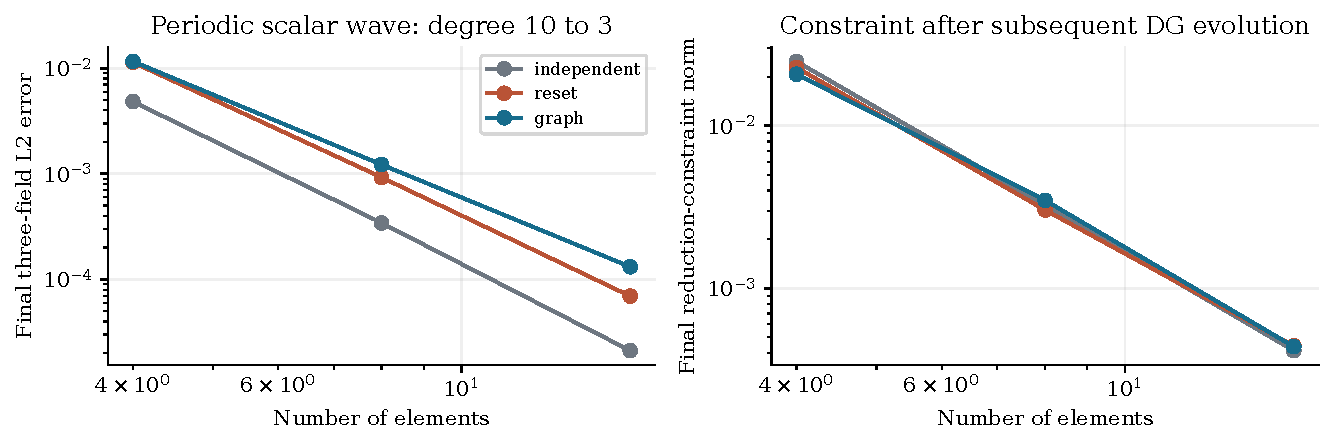
\includegraphics[width=\linewidth]{../figures/dg.pdf}
\caption{Subsequent evolution can reverse the impression from an instantaneous constraint check. Field error (left) favors independent projection; final local constraint norms (right) do not have a consistent ordering. All three methods improve with spatial refinement in this test.}\label{fig:dg}
\end{figure}

\section{Implications for adaptive wave software}
The two-trace result provides a transfer diagnostic that can accompany an existing modal error estimator. At each proposed degree, a code can compute the expected injection before altering the state, compare it with a specified constraint budget, and retain the existing approximation-error criterion. Both conditions must be tested: the cancellation example rules out using injection alone. For a source with existing inconsistency, \eqref{eq:oldnew} separates retained old constraint from newly injected constraint. Such separation can help distinguish errors introduced by adaptivity from errors generated during evolution.

The result suggests a modest software contribution for spectral wave codes: a reproducible unit-test fixture and an element-local observer of predicted versus measured transfer injection. A SpECTRE implementation would need to match its actual projection, modal normalization, quadrature, and mesh maps \cite{spectre}. The present code does not modify SpECTRE and provides no evidence of a defect in its current implementation. Exact unweighted \(L^2\) projection is an assumption of the proof, not a description asserted for every production regridding path. Gauss--Lobatto mass lumping must not silently replace the exact mass in \eqref{eq:mass}; in particular, its highest-mode norm differs from the exact integral.

Curved maps and spatially varying weights also require care. For a physical derivative \(a(x)\partial_x\), integration by parts against a test function introduces derivatives of \(a\) in the interior. The simple orthogonality argument used in Theorem~\ref{thm:trace} no longer removes all such terms in general. A mapped-element extension must derive its own interior correction. Similarly, the first-order generalized harmonic reduction constraints are only one part of the Einstein constraint system. Satisfying their linear affine analogue does not enforce the gauge, Hamiltonian, momentum, or full nonlinear constraints.

Potential engineering applications include diagnostics for adaptive simulation and derivative-aware checkpoint compression in wave-based inverse problems. The exact indicator could identify transfers requiring closer scrutiny, while the counterexamples give regression tests for a numerical-software quality service. These are plausible uses, not measured commercial outcomes. This study contains no market-size estimate, customer validation, patentability finding, or demonstrated reduction in production compute cost. Its practical value is an explicit, inexpensive consistency check whose limitations are also explicit.

\section{Conclusions}
For exact Legendre \(p\)-coarsening on an affine interval, two discarded-tail traces determine the complete derivative-constraint injection. The resulting quadratic norm and finite-band singular values give exact local diagnostics. Cancellation makes this injection nonmonotonic in retained degree and separates it from approximation accuracy. The same traces produce a cached-response specialization of standard graph projection for consistent data. That projection is contractive in its specified pair norm; derivative reset need not be.

The scalar-wave experiments show why these properties should be used diagnostically rather than as a blanket recommendation to project onto compatibility after every transfer. Ordinary fieldwise projection can yield smaller later solution error, and local consistency can be lost through subsequent interface evolution. A useful next validation step is therefore to instrument the actual transfer and interface operators of a numerical-relativity code, including mapped elements and its full constraint norm, before evaluating any effect on waveform accuracy. The present results supply exact reference identities and counterexamples for that investigation.

\paragraph{Code and data availability.}
The repository at \url{https://github.com/shi1720/legendre-constraint-coarsening} contains the executable experiments, nine automated tests, raw numerical results, figures, and this manuscript. Code is released under the MIT license. The manuscript is an unpublished technical study; no publication or presentation acceptance is implied.

\begin{thebibliography}{10}\small
\bibitem{lindblom} L. Lindblom, M. A. Scheel, L. E. Kidder, R. Owen, and O. Rinne. A new generalized harmonic evolution system. \emph{Classical and Quantum Gravity} 23 (2006), S447--S462. \href{https://doi.org/10.1088/0264-9381/23/16/S09}{doi:10.1088/0264-9381/23/16/S09}.
\bibitem{szilagyi} B. Szilagyi. Key elements of robustness in binary black hole evolutions using spectral methods. \emph{International Journal of Modern Physics D} 23 (2014), 1430014. \href{https://doi.org/10.1142/S0218271814300146}{doi:10.1142/S0218271814300146}.
\bibitem{kidder} L. E. Kidder et al. SpECTRE: A task-based discontinuous Galerkin code for relativistic astrophysics. \emph{Journal of Computational Physics} 335 (2017), 84--114. \href{https://doi.org/10.1016/j.jcp.2016.12.059}{doi:10.1016/j.jcp.2016.12.059}.
\bibitem{spectre} SpECTRE Collaboration. Spectral namespace reference. \url{https://spectre-code.org/namespaceSpectral.html}. Accessed 17 October 2026.
\bibitem{holst} M. Holst, L. Lindblom, R. Owen, H. P. Pfeiffer, M. A. Scheel, and L. E. Kidder. Optimal constraint projection for hyperbolic evolution systems. \emph{Physical Review D} 70 (2004), 084017. \href{https://doi.org/10.1103/PhysRevD.70.084017}{doi:10.1103/PhysRevD.70.084017}.
\bibitem{rapisarda} P. Rapisarda, H. J. van Waarde, and M. K. Camlibel. Orthogonal polynomial bases for data-driven analysis and control of continuous-time systems. \emph{IEEE Transactions on Automatic Control} 69 (2024), 4307--4319. \href{https://doi.org/10.1109/TAC.2023.3321214}{doi:10.1109/TAC.2023.3321214}.
\bibitem{huynh} H. T. Huynh. On formulations of discontinuous Galerkin and related methods for conservation laws. NASA/TM-2014-218135 (2014). \url{https://ntrs.nasa.gov/citations/20140009969}.
\bibitem{shen} J. Shen. Efficient spectral-Galerkin method I. Direct solvers of second- and fourth-order equations using Legendre polynomials. \emph{SIAM Journal on Scientific Computing} 15 (1994), 1489--1505. \href{https://doi.org/10.1137/0915089}{doi:10.1137/0915089}.
\bibitem{canuto} C. Canuto, R. H. Nochetto, and M. Verani. Contraction and optimality properties of adaptive Legendre--Galerkin methods: The one-dimensional case. \emph{Computers \& Mathematics with Applications} 67 (2014), 752--770. \href{https://doi.org/10.1016/j.camwa.2013.05.025}{doi:10.1016/j.camwa.2013.05.025}.
\end{thebibliography}
\end{document}
